\begin{task}{344}
Перечислите все попарно неизоморфные связные простые графы на шести вершинах, в которых ровно три блока.
\end{task}

\begin{solution}
Разобьем графы на группы, для простоты и алгоритмичности перебора:
\begin{figure}[H]
  \centering
  \begin{subfigure}[a]{0.24\linewidth}
    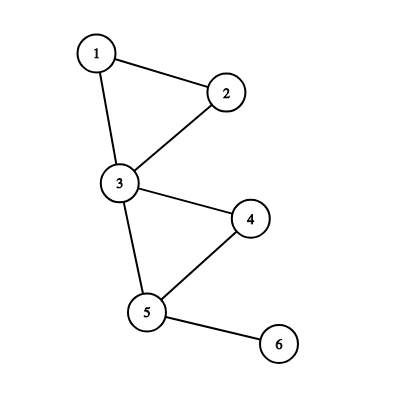
\includegraphics[width=\linewidth]{_img/344/01.png}
  \end{subfigure}
  \begin{subfigure}[a]{0.24\linewidth}
    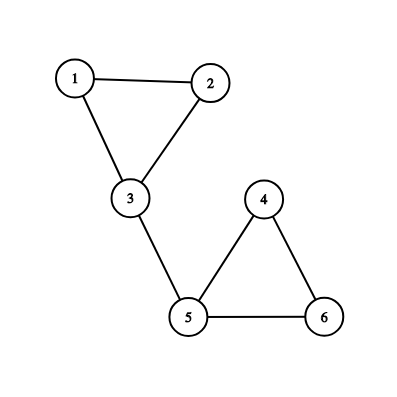
\includegraphics[width=\linewidth]{_img/344/02.png}
  \end{subfigure}
  \begin{subfigure}[a]{0.24\linewidth}
    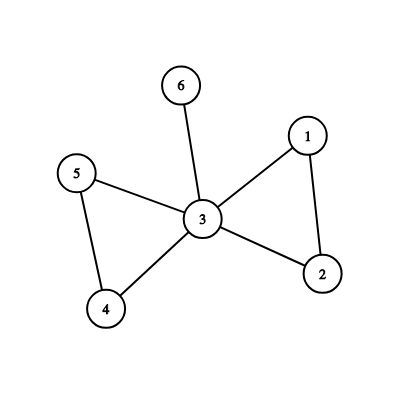
\includegraphics[width=\linewidth]{_img/344/03.png}
  \end{subfigure}
  \caption{Два треугольника и ребро.}
\end{figure}

\begin{figure}[H]
  \centering
  \begin{subfigure}[a]{0.24\linewidth}
    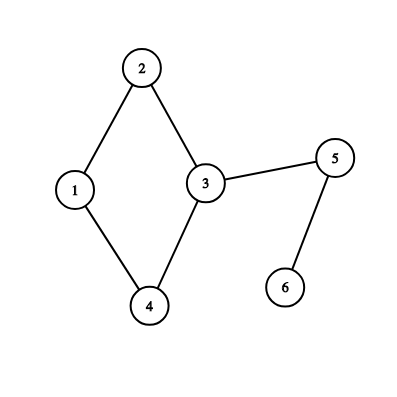
\includegraphics[width=\linewidth]{_img/344/04.png}
  \end{subfigure}
  \begin{subfigure}[a]{0.24\linewidth}
    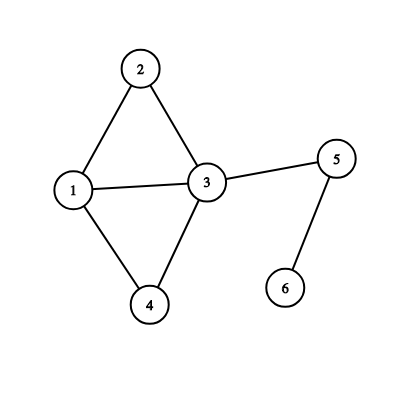
\includegraphics[width=\linewidth]{_img/344/05.png}
  \end{subfigure}
  \begin{subfigure}[a]{0.24\linewidth}
    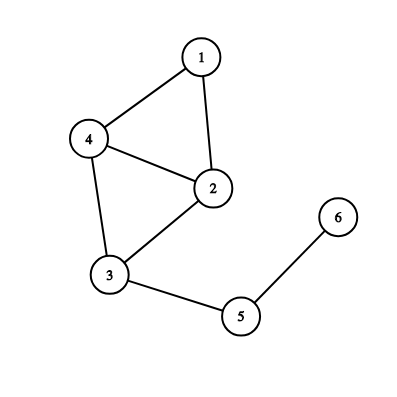
\includegraphics[width=\linewidth]{_img/344/06.png}
  \end{subfigure}
  \begin{subfigure}[a]{0.24\linewidth}
    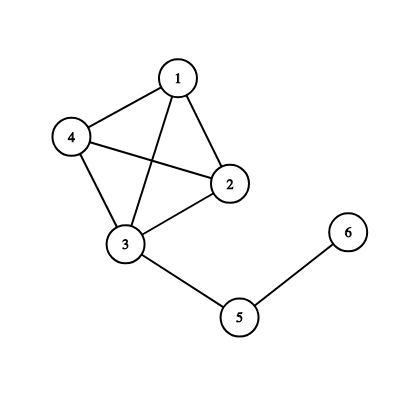
\includegraphics[width=\linewidth]{_img/344/07.png}
  \end{subfigure}
  \caption{Квадрат и два последовательных ребра.}
\end{figure}

\begin{figure}[H]
  \centering
  \begin{subfigure}[a]{0.24\linewidth}
    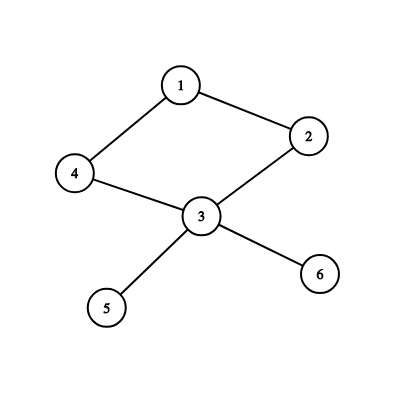
\includegraphics[width=\linewidth]{_img/344/08.png}
  \end{subfigure}
  \begin{subfigure}[a]{0.24\linewidth}
    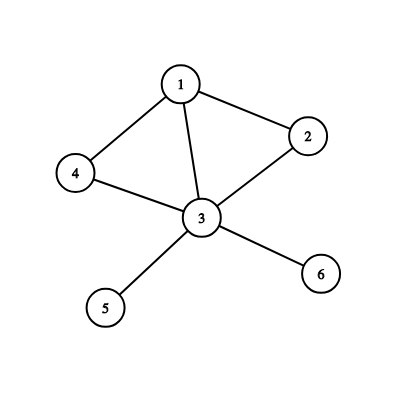
\includegraphics[width=\linewidth]{_img/344/09.png}
  \end{subfigure}
  \begin{subfigure}[a]{0.24\linewidth}
    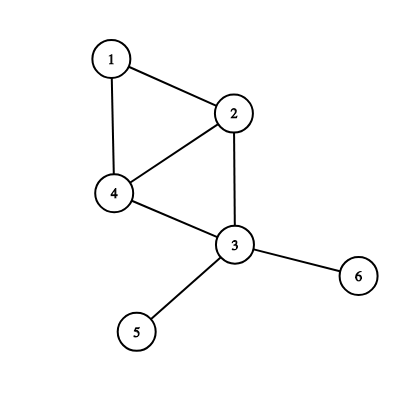
\includegraphics[width=\linewidth]{_img/344/10.png}
  \end{subfigure}
  \begin{subfigure}[a]{0.24\linewidth}
    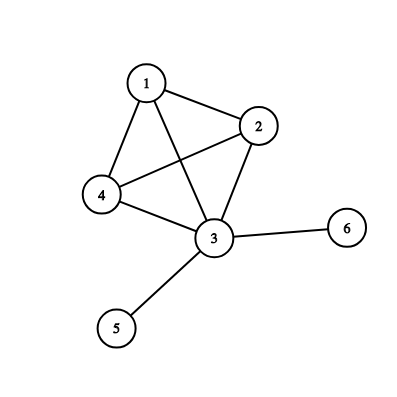
\includegraphics[width=\linewidth]{_img/344/11.png}
  \end{subfigure}
  \caption{Квадрат и два инцидентных ребра.}
\end{figure}

\begin{figure}[H]
  \centering
  \begin{subfigure}[a]{0.24\linewidth}
    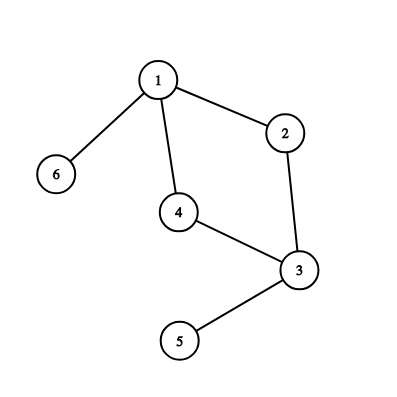
\includegraphics[width=\linewidth]{_img/344/12.png}
  \end{subfigure}
  \begin{subfigure}[a]{0.24\linewidth}
    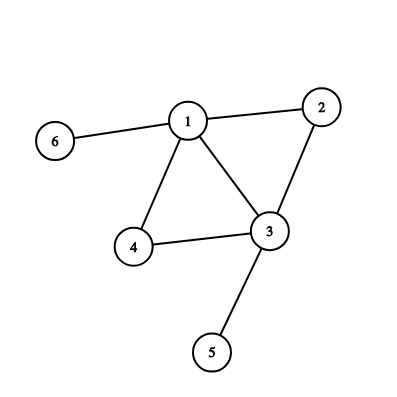
\includegraphics[width=\linewidth]{_img/344/13.png}
  \end{subfigure}
  \begin{subfigure}[a]{0.24\linewidth}
    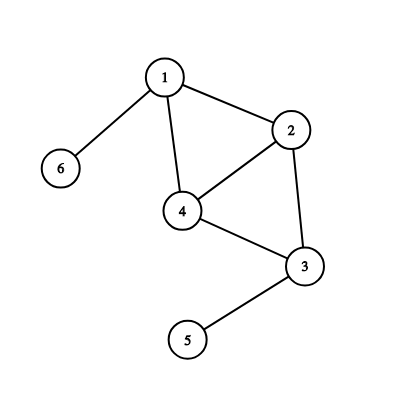
\includegraphics[width=\linewidth]{_img/344/14.png}
  \end{subfigure}
  \begin{subfigure}[a]{0.24\linewidth}
    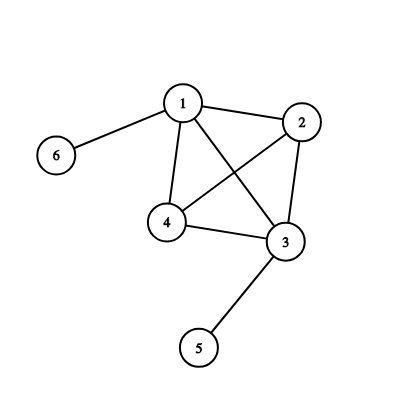
\includegraphics[width=\linewidth]{_img/344/15.png}
  \end{subfigure}
  \caption{Квадрат и два диаметрально противоположных ребра.}
\end{figure}

\begin{figure}[H]
  \centering
  \begin{subfigure}[a]{0.24\linewidth}
    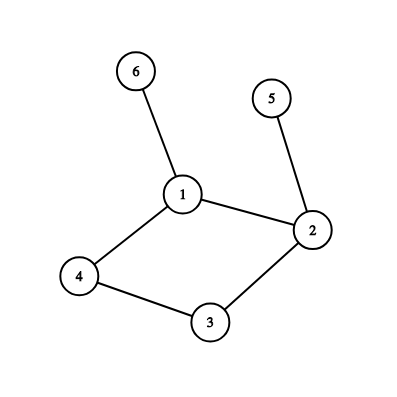
\includegraphics[width=\linewidth]{_img/344/16.png}
  \end{subfigure}
  \begin{subfigure}[a]{0.24\linewidth}
    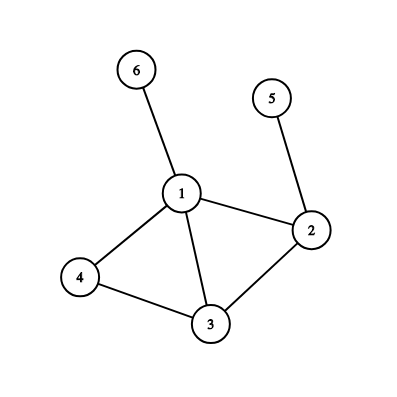
\includegraphics[width=\linewidth]{_img/344/17.png}
  \end{subfigure}
  \caption{Квадрат и два ребра.}
\end{figure}

Таким образом, искомых графов всего семнадцать.
\end{solution}